\clearpage

\section{CAPEX}
\begin{tcolorbox}	
\begin{tabular}{p{2.75cm} p{0.2cm} p{10.5cm}} 	
\textbf{Student Name}  &:& Tiago Esteves    (October 03, 2017 - )\\
\textbf{Goal}          &:& Implement of the ILP model to obtain the best possible CAPEX of a given network.
\end{tabular}
\end{tcolorbox}
\vspace{11pt}

The cost of a telecommunications network can be divided into CAPEX and OPEX.
CAPEX is the amount of money needed to set up and install a particular network.
OPEX is the amount of money needed to run this network as well as its maintenance and operation over time.
In this section we will only focus on CAPEX, that is, the costs of installing a particular network.
As we know the telecommunications networks are made up of links and nodes, so it is possible to define the CAPEX as being the sum of the cost of links and cost of nodes.
This can be said that the value of CAPEX is given by the equation \ref{Capex}.

\begin{equation}
C_C = C_L + C_N
\label{Capex}
\end{equation}


\begin{itemize}
\item{$C_C$				$\rightarrow$	CAPEX cost}
\item{$C_L$				$\rightarrow$	Link cost}
\item{$C_N$				$\rightarrow$	Node cost}
\end{itemize}


\vspace{11pt}
For this calculation first let's focus on the cost of the links and for this we have to take into account the figure \ref{link_design} where we can see the design of a link. In this figure we can see that a link consists of two optical line terminals (one at each end), it also has several amplifiers (this number depends on the length of the link) placed at a certain distance (span) and finally it also consists of several optical channels each with a certain wavelength.

\begin{figure}[h!]
\centering
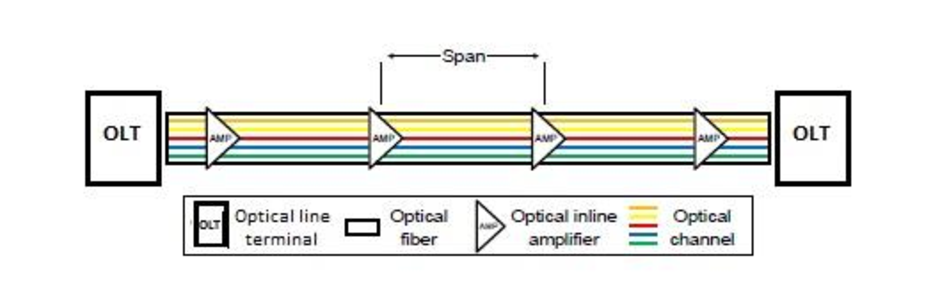
\includegraphics[width=\textwidth]{sdf/ILP/figures/link_design}
\caption{Design of a link.}
\label{link_design}
\end{figure}

\newpage
Thus, through the previous image, we can conclude that the link cost is calculated by the equation \ref{Capex_Link}.

\begin{equation}
C_L = \sum_{i=1}^N \sum_{j=i+1}^N L_{ij} \left( 2 \gamma_0^{OLT} + 2 \gamma_1^{OLT} \tau W_{ij} + N^R_{ij} c^R \right)
\label{Capex_Link}
\end{equation}

\begin{itemize}
\item{$C_L$				$\rightarrow$	Links cost}
\item{$i$               $\rightarrow$   Index for start node of a physical link}
\item{$j$               $\rightarrow$   Index for end node of a physical link}
\item{$N$				$\rightarrow$	Total number of nodes}
\item{$L_{ij}$			$\rightarrow$	Binary variable indicating if link between the nodes $i$ and $j$ is used}
\item{$\gamma_0^{OLT}$	$\rightarrow$	OLT cost in euros}
\item{$\gamma_1^{OLT}$	$\rightarrow$	Transponder cost in euros}
\item{$\tau$		    $\rightarrow$	Line bit-rate}
\item{$W_{ij}$          $\rightarrow$   Number of optical channels in link $i$ $j$}
\item{$N^R_{ij}$    	$\rightarrow$	Number of optical amplifiers in link $i$ $j$}
\item{$c^R$				$\rightarrow$	Optical amplifiers cost in euros}
\end{itemize}


The next step is to take into account the cost of the nodes, but for this we must first know how a node is constituted. The nodes have an electrical part and an optical part so we can conclude that the cost of the nodes is given by the sum of these two parts thus obtaining the equation \ref{Capex_Node}.

\begin{equation}
C_N = C_{EXC} + C_{OXC}
\label{Capex_Node}
\end{equation}

\vspace{11pt}
In relation to the electric part we can see the figure \ref{exc_design} where it shows its constitution.

\begin{figure}[h!]
\centering
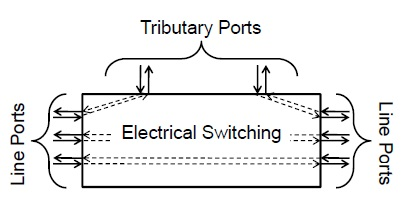
\includegraphics[width=8cm]{sdf/ILP/figures/exc_design}
\caption{Design of a electrical switching.}
\label{exc_design}
\end{figure}


Thus, through the previous image, we can conclude in a simple way that the electric cost is the sum of the fixed cost of the electrical connection with the total cost of all the electric ports.
Therefore the electric cost is given by equation \ref{Capex_Node_EXC}.

\begin{equation}
C_{EXC} = \sum_{n=1}^{N} N_{exc,n} \left( \gamma_{e0} + \sum_{c=-1}^B \gamma_{e1,c} P_{exc,c,n} \right)
\label{Capex_Node_EXC}
\end{equation}

\begin{itemize}
\item{$C_{EXC}$			$\rightarrow$	Electrical cost}
\item{$N$				$\rightarrow$	Total number of nodes}
\item{$N_{exc,n}$		$\rightarrow$	Binary variable indicating if node $n$ is used}
\item{$\gamma_{e0}$ 	$\rightarrow$	EXC cost in euros}
\item{$B$           	$\rightarrow$	|100G line, 1.25G tributary, 2.5G tributary, 10G tributary, 40G tributary, 100G tributary|}
\item{$c$               $\rightarrow$   Index for bit rate (-1; 0; 1; 2; 3; 4)}
\subitem{$-1$           $\rightarrow$   100 Gbits/s line bit-rate (long-reach port)}
\subitem{$0$            $\rightarrow$   1.25 Gbits/s tributary bit-rate (short-reach port)}
\subitem{$1$            $\rightarrow$   2.5 Gbits/s tributary bit-rate (short-reach port)}
\subitem{$2$            $\rightarrow$   10 Gbits/s tributary bit-rate (short-reach port)}
\subitem{$3$            $\rightarrow$   40 Gbits/s tributary bit-rate (short-reach port)}
\subitem{$4$            $\rightarrow$   100 Gbits/s tributary bit-rate (short-reach port)}
\item{$\gamma_{e1,c}$	$\rightarrow$	EXC port cost in euros with bit-rate $B$ and with a given transceiver reach}
\item{$P_{exc,c,n}$	    $\rightarrow$	Number of ports of the electrical switch}
\end{itemize}

\vspace{11pt}
In relation to the optical part we can see the figure \ref{oxc_design} where it shows its constitution.

\begin{figure}[h!]
\centering
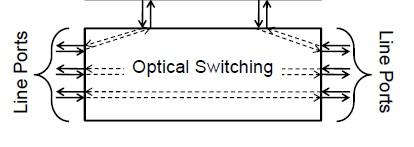
\includegraphics[width=8cm]{sdf/ILP/figures/oxc_design}
\caption{Design of a optical switching.}
\label{oxc_design}
\end{figure}


Thus, through the previous image, we can conclude in a simple way that the electric cost is the sum of the fixed cost of the optical connection with the total cost of all the optical ports.
Therefore the optical cost is given by equation \ref{Capex_Node_OXC}.

\begin{equation}
C_{OXC} = \sum_{n=1}^{N} N_{oxc,n} \left( \gamma_{o0} + \gamma_{o1} P_{oxc,n} \right)
\label{Capex_Node_OXC}
\end{equation}

\begin{itemize}
\item{$C_{OXC}$			$\rightarrow$	Optical cost}
\item{$N$				$\rightarrow$	Total number of nodes}
\item{$N_{oxc,n}$		$\rightarrow$	Binary variable indicating if node $n$ is used}
\item{$\gamma_{o0}$ 	$\rightarrow$	OXC cost in euros}
\item{$\gamma_{o1}$ 	$\rightarrow$	OXC port cost in euros }
\item{$P_{oxc,n}$	    $\rightarrow$	Number of ports of the optical switch}
\end{itemize}


\vspace{10pt}
We have to take into account that the calculated value for the variable $P_{exc,c,n}$ and $P_{oxc,n}$ will depend on the mode of transport used (opaque, transparent or translucent) but later on it will be explained how these values are calculated for each specific transport mode.\\
To obtain the best possible value, it will be necessary to minimize the cost of the capex mentioned above so that we can obtain the objective function.


